\documentclass{beamer}
\usepackage{HECbeamer}
\usepackage{icomma}
\newcommand{\AIC}{\textsf{AIC}}
\newcommand{\BIC}{\textsf{BIC}}
% \usepackage{pgfpages}
% \pgfpagesuselayout{4 on 1}[letterpaper, landscape, border shrink=5mm]
\title[\color{white}{MATH 60604 \S~4b - Régression logistique}]{\texorpdfstring{MATH 60604 \\Modélisation statistique \\ \S~4b - Régression logistique}{MATH 60604 \\Modélisation statistique \\ \S~4b - Régression logistique}}
\author{Léo Belzile}
\institute{HEC Montréal\\
Département de sciences de la décision}
\date{} 

\begin{document}
\frame{\titlepage}

\begin{frame}[fragile]
\frametitle{Modèles linéaires généralisés pour données binaires}

\bi
\item  Si notre variable réponse est binaire, on peut supposer que $Y_i $ suit une loi Bernoulli de paramètre $\pi_i$, $Y_i\sim \mathsf{Bin}(\pi_i) $, où
\[\pi_i= \P{Y_i=1 \mid \mathbf{X}_i}=\E{Y_i \mid \mathbf{X}_i}.\]
\item La fonction de liaison la plus courante pour les réponses binaires est la fonction \alert{logit} 
\begin{align*}
g(z)\coloneqq\logit(z)=\ln\left(\frac{z}{1-z}\right).
\end{align*}
soit la \textbf{fonction quantile de la loi logistique} qui ici relie $\E{Y_i\mid \mathbf{X}_i}=\pi_i(\mathbf{X}_i)$ et $\eta_i$.
\ei
\end{frame}



\begin{frame}[fragile]
\frametitle{Fonction de liaison logit}
\bi
\item Le modèle logistique spécifie
\begin{align*}
\eta_i=\ln\left(\frac{\pi_i}{1-\pi_i}\right)=\beta_0+ \beta_1 \mathrm{X}_{i1} + \cdots + \beta_p \mathrm{X}_{ip}.
\end{align*}
\item Ce modèle peut être exprimé sur l'échelle de la moyenne à l'aide de la fonction inverse de \alert{logit} (expit), 
\begin{align*}
\E{Y_i \mid \mathbf{X}_i}=\pi_i=\frac{\exp(\beta_0+ \beta_1  \mathrm{X}_{i1} + \cdots + \beta_p \mathrm{X}_{ip})}{1+\exp(\beta_0+ \beta_1  \mathrm{X}_{i1} + \cdots + \beta_p \mathrm{X}_{ip})}.
\end{align*}
\item Cela donne une expression pour la moyenne $\pi_i=\E{Y_i\mid \mathbf{X}_i}$ en fonction des variables explicatives $\mathbf{X}_i$, mais\ldots
\bi
 
\item à quoi ressemble cette fonction?
\item que nous apprend-elle sur la relation entre $\pi_i$ et $\eta_i$ (et donc $\mathbf{X}_{i}$)?
\ei
\ei
\end{frame}

\begin{frame}[fragile]
\frametitle{Fonction de répartition logistique}



\begin{center}
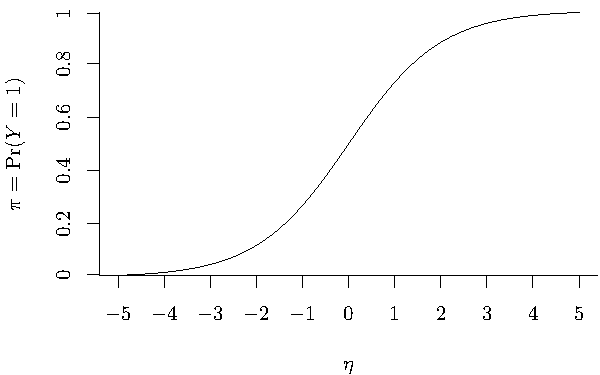
\includegraphics[width = 0.7\linewidth]{img/c4/08-glm-logisticcdf}
\end{center}
\bi
\item On voit que $\pi$ est une \textbf{fonction croissante} de $\eta=\beta_0 + \sum_{j=1}^p \beta_j \mathrm{X}_{j}$.
{\small \bi 
\item Si $\beta_j$ est positif et $\mathrm{X}_{j}$ augmente, $\P{Y=1}$ augmente aussi.  
\item Si $\beta_j$ est négatif et  $\mathrm{X}_{j}$ augmente, $\P{Y=1}$ diminue. 
\ei
}
\item La relation entre $\P{Y=1}$ et $\eta$ (et donc aussi $\mathrm{X}_{j}$) est \alert{nonlinéaire}.
\ei
\end{frame}
% 
% \begin{frame}[fragile]
% \frametitle{Interprétation des coefficients de la régression logistique}
% \begin{tcolorbox}[colback=white, colframe=hecblue, title=Interprétation générale]
% \bi
% \item Si $\beta_j$ est positif, plus la valeur de $\beta_j$ est grande, plus l'augmentation de la probabilité que $Y=1$ \alert{augmente} avec $\mathrm{X}_j$.
% \item Si $\beta_j$ est négative, plus la valeur de $|\beta_j|$ augmente, plus l'augmentation de la probabilité que  $Y=1$ \textbf{décroît} avec $\mathrm{X}_j$.
% \ei
% \end{tcolorbox}
% 
% \end{frame}


\begin{frame}[fragile]
\frametitle{Interprétation des paramètres de la régression logistique}
\bi
\item Quantifier les effets des paramètres $\bs{\beta}$ de la régression logistique est compliqué à cause de la nonlinéarité.
\item L'effet des coefficients est en terme de \alert{cote} et de  \alert{rapports de cote}.
\item Soit $\pi=\P{Y=1\mid \mathrm{X}_1, \ldots, \mathrm{X}_p}$ et le modèle de régression logistique
\begin{align*}
\ln\left(\frac{\pi}{1-\pi}\right)=\beta_0+ \beta_1 \mathrm{X}_1 + \cdots + \beta_p\mathrm{X}_p.
\end{align*}
\item Si on prend l'exponentielle de chaque côté de l'équation précédente, on obtient
\begin{align*}
\mathrm{cote}(Y\mid \mathbf{X}) = \frac{\pi(\mathbf{X})}{1-\pi(\mathbf{X})}=\exp(\beta_0+ \beta_1 \mathrm{X}_1 + \cdots + \beta_p\mathrm{X}_p),
\end{align*}
où $\pi(\mathbf{X})/\{1-\pi(\mathbf{X})\}$ est la cote de $\P{Y=1 \mid \mathbf{X}}$ par rapport à $\P{Y=0 \mid\mathbf{X}}$.
\ei
\end{frame}
\begin{frame}[fragile]
\frametitle{Cote}
\bi
\item L'utilisation de la fonction de liaison logit donne un modèle pour le \textbf{log de la cote}.

\item La cote pour une variable binaire $Y$ est le rapport
\begin{align*}
 \mathrm{cote}(\pi) = \frac{\pi}{1-\pi} = \frac{\P{Y=1}}{\P{Y=0}}.
\end{align*}

\item Par exemple, une cote de $4$ signifie que la probabilité de  $Y=1$ est quatre fois plus élevée que la probabilité de $Y=0$. 
\item Une cote de $0,25$ à l'inverse veut dire que la probabilité de $Y=1$ est seulement le quart de celle pour $Y=0$, ou encore que la probabilité de $Y=0$ est quatre fois plus élevée que celle pour $Y=1$.
\ei

\begin{tabular}{lccccccccc}
\toprule
 $\P{Y=1}$& $0,1$ & $0,2$ & $0,3$ & $0,4$ & $0,5$ & $0,6$& $0,7$ & $ 0,8$& $0,9$\\
 cote & $0,11$ & $0,25$ & $0,43$ & $0,67$ & $1$ &$1,5$ & $2,33$ & $4$ & $9$\\
 cote (frac.) & $\frac{1}{9}$ & $\frac{1}{4}$
 & $\frac{3}{7}$ & $\frac{2}{3}$ & $1$ & $\frac{3}{2}$ & $\frac{7}{3}$ & $4$ & $9$\\
 \bottomrule
 
\end{tabular}
\end{frame}

\begin{frame}[fragile]
\frametitle{Interprétation de l'ordonnée à l'origine en termes de cote}
\bi
\item Si $\mathrm{X}_1=\cdots = \mathrm{X}_p=0$, il est clair que
\begin{align*}
\mathrm{cote}(Y\mid \mathbf{X}=\bs{0}_p) = \exp(\beta_0)
\end{align*}
et
\begin{align*}
\P{Y=1\mid  \mathbf{X}=\bs{0}_p} = \frac{\exp({\beta_0})}{1+\exp({\beta_0})}
\end{align*}
représente la probabilité que $Y=1$ quand $\mathbf{X}=\bs{0}_p$.
\item Comme pour la régression linéaire, $\mathrm{X}_1=\cdots =\mathrm{X}_p=0$ peut être impossible; dans ce cas, $\beta_0$ ne s'interprète pas.
\ei
\end{frame}

\begin{frame}[fragile]
\frametitle{Interprétation des paramètres en termes de rapports de cotes}
On considère pour faire simple un modèle logistique de la forme
\[\logit(\pi) = \beta_0 + \beta_1x.\]
Le facteur $\exp(\beta_1)$ est le changement dans la cote quand $\mathrm{X}$ augmente d'une unité,
\begin{align*}
\mathrm{cote}(Y \mid  \mathrm{X}=x+1) = \exp(\beta_1) \times \mathrm{cote}(Y \mid  \mathrm{X}=x).
\end{align*}
\bi
\item Si $\beta_1=0$, le rapport des cotes vaut un: $\mathrm{X}$ n'impacte pas la cote de $Y$
\item Si $\beta_1$ est positif, le rapport des cotes $\exp(\beta_1)$ excède un: si $\mathrm{X}$ croît, la cote de $Y$ augmente.
\item Si $\beta_1$ est négatif, le rapport des cotes $\exp(\beta_1)$ est inférieur à un: si $\mathrm{X}$ croît, la cote de  $Y$ décroît.

\ei 

\footnotesize{Quand il y a plusieurs variables explicatives, l'interprétation de $\beta_1$ est identique, mais elle n'est valide que quand \alert{toutes les autres variables explicatives sont égales par ailleurs.}

}

\end{frame}
\begin{frame}[fragile]
\frametitle{Interprétation de $\beta_k$ en terme de rapport de cote}

Dans le modèle logistique,  le \alert{rapport de cotes} quand $\mathrm{X}_k=x_k+1$ versus $\mathrm{X}_k=x_k$ quand $\mathrm{X}_j=x_j$ $(j=1, \ldots, p, j \neq k)$ est
{\small
\begin{align*}
\frac{\mathrm{cote}(Y \mid  \mathrm{X}_k=x_k+1, \mathrm{X}_j=x_j, j\neq k)}{\mathrm{cote}(Y \mid \mathrm{X}_k=x_k, \mathrm{X}_j=x_j, j \neq k)}&=\frac{\exp\left(\beta_0+ \sum_{j=1}^p\beta_j x_j + \beta_k \right)}{\exp\left(\beta_0+ \sum_{j=1}^p\beta_j x_j \right)}\\
&= \exp(\beta_k).
\end{align*}
}

Quand $\mathrm{X}_k$ augmente d'une unité \textbf{et que la valeur de toutes les autres covariables est constante}, la cote de $Y$ est multipliée par un $\exp(\beta_k)$.
\bi 
\item La cote augmente si $\exp(\beta_k) >1$, c'est-à-dire si $\beta_k>0$.
\item La cote diminue si $\exp(\beta_k) < 1$,  c'est-à-dire si $\beta_k<0$.
\ei
\end{frame}


\end{document}
